\chapter{Installation}
\label{chap:inst}

Für die Installation von ERPNext werden seitens Frappé diverse Möglichkeiten angeboten. Diese stehen alle inklusive Anleitung auf ihrem GitHub-Repository zur Verfügung (\vgl \cite{GhBench}).

Generell weist Frappé als lauffähige Systeme für den Betrieb von ERPNext alle Betriebssysteme außer Windows aus. Grund hierfür ist das \gls{cli} der Software, das unter Microsofts Betriebssystem nicht lauffähig zu sein scheint. Genauere Erläuterungen dafür werden vom Hersteller nicht geliefert. Als präferierte Systeme werden auf Linux-Seite Debian, Ubuntu und CentOS vorgeschlagen, die als besonders gut getestete Systeme gelten. Darüber hinaus werden noch Arch Linux und macOS genannt. \\
Von unserer Seite wurde für die manuelle Installation und das Installationsskript zu Testzwecken anfangs die Linux Distribution Xubuntu in der neuesten Version (18.04, \glqq Bionic Beaver\grqq) verwendet. Da sich diese Version jedoch als nicht geeignet herausstellte – dazu im nächsten Abschnitt mehr – wurde auf Xubuntu in einer älteren Version (16.04, \glqqXenial Xerus\grqq) zurückgegriffen.
 
Für die 60-minütige Präsentation wurde ERPNext per Installationsskript auch auf einem \gls{vps} eingerichtet. Dieser verfügt über zwei virtuelle Kerne, 2 GB DDR3-Arbeitspeicher, 10 GB SSD-Festplattenspeicher und das Betriebssystem Debian (8.10, Jessie). Diese Konfiguration erwies sich schon als vollkommen ausreichend für unsere Zwecke.

\section{Installationsskript}
Die einfachste Form der Installation auf einem Produktivsystem stellt das \glqq Easy Install\grqq-Python-Skript dar. Dafür benötigt das System lediglich die Programmiersprache Python in Version 2.7, was bei allen gängigen Unix-Systemen der Fall sein dürfte. \\
Offiziell werden die Betriebssysteme Ubuntu 16.04, CentOS 7 und höher, sowie Debian 8 und höher für das Skript unterstützt. Bei einem genaueren Blick in die Python-Datei fällt aber auf, dass auch die Darwin-Plattform, genauer gesagt macOS in den Versionen 10.9 - 10.12 bedacht wurde.\\
Da ERPNext ursprünglich auf einem Ubuntu-Derivat in der Version 18.04 installiert werden sollte, schlug der Installer erwartungsgemäß fehl (\vgl Abbildung \ref{fig:fehlInst}).
\begin{figure}[H]
  \centering
  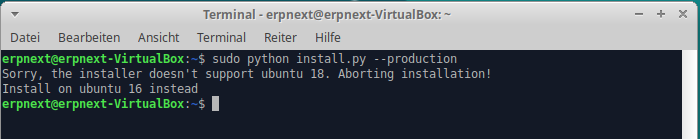
\includegraphics[width=\textwidth]{Bilder/Fehlgeschlagene_Installation.PNG}
  \caption{Fehlgeschlagene Installation aufgrund der OS-Version}
  \label{fig:fehlInst}
\end{figure}
Wieso hierbei nur ein zwei Jahre altes Betriebssystem\footnote{\Vgl \cite{Ubuntu}. Die Ursprungsversion von 16.04 wurde bereits am 21. April 2016 veröffentlicht. Da es sich jedoch um eine \gls{lts} Versionsnummer handelt, erhält die normale Ubuntu-Version Updates bis 2021, das Derivat Xubuntu bis 2019 (\vgl \cite{Xubuntu16}).}  unterstützt wird, erscheint fraglich.\\
Auch die Änderung einer Codezeile im Python-Skript brachte nicht den gewünschten Erfolg und das Programm wurde mit einer Fehlermeldung abgebrochen (\vgl Abbildung \ref{fig:fehlInst2}). Nach dem Zurückgreifen auf die unterstützte Version 16.04 verlief die Installation ohne Probleme.
\begin{figure}
  \centering
  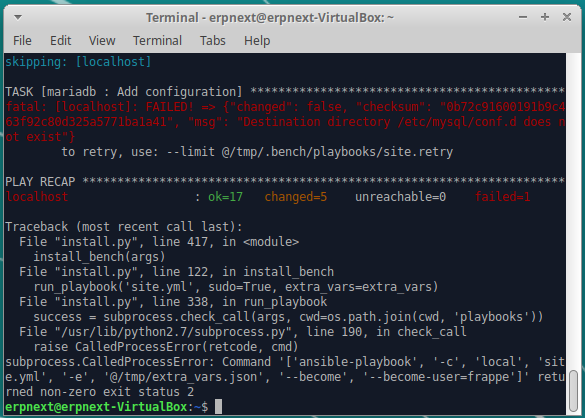
\includegraphics[width=\textwidth]{Bilder/Fehlgeschlagene_Installation_2.PNG}
  \caption{Fehlgeschlagene Installation aufgrund eines fehlenden Ordners}
  \label{fig:fehlInst2}
\end{figure}
An dieser Stelle hat der Nutzer auch die Wahl zwischen einer Entwickler- oder einer Produktiv-Installation. Aus einem Forums-Diskussionsbeitrag geht hervor, dass der Unterschied darin liegt, dass lediglich im sogenannten\glqq developer mode\grqq\ neue Vorlagen für beispielsweise Reports erstellt werden können. Die Produktiv-Installation hingegen lässt lediglich Änderungen zu, die über das Frontend von ERPNext gesteuert werden können (\vgl \cite{ProdVsDev}). Darüber hinaus werden bei der Produktiv-Variante bereits diverse Management-Tools automatisch aktiviert. \\
Zudem können beide Installationen mittels Parameter von einem neuen User angelegt werden, sodass ERPNext/Frappé Bench nicht direkt vom Root-User installiert werden muss.
Somit reduziert sich die ganze Installation beispielsweise auf:
\begin{minted}[linenos=true,escapeinside=||]{bash}
wget https://raw.githubusercontent.com/frappe/bench/master/playbooks/install.py
sudo python install.py --production --user erpnextUser
\end{minted}
Dabei wird das Skript zuerst heruntergeladen und dann im Produktiv-Modus für den Benutzer \glqq erpnextUser\grqq\ gestartet. \\
Während der Ausführung des Skripts werden alle benötigten Abhängigkeiten heruntergeladen und konfiguriert. Dazu zählen unter anderem diverse Python-Tools, MariaDB für die Datenhaltung, Redis als Key-Value-Store und Nginx als Webserver. Zudem werden verschiedene Parameter abgefragt, wie zum Beispiel das Datenbank Root-Passwort oder das Administrator-Passwort für ERPNext. Hierbei fällt positiv auf, dass der Benutzer immer über den Stand der verschiedenen Installationsschritte auf dem Laufenden gehalten wird (\vgl Abbildung \ref{fig:aktInst}). Negativ – wenn auch sicherlich nützlich – ist eine angelegte Textdatei, die die zuvor angelegten Passwörter im Klartext enthält.
\begin{figure}[H]
  \centering
  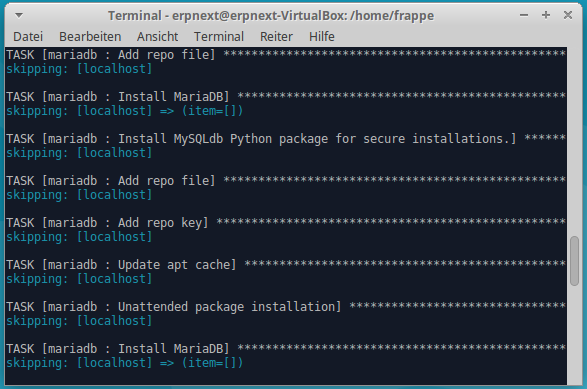
\includegraphics[width=\textwidth]{Bilder/Aktueller_Stand_Installation.PNG}
  \caption{Aktueller Stand der Installation}
  \label{fig:aktInst}
\end{figure}

\section{Manuelle Installation}
Auch die manuelle Installation ist sehr übersichtlich gehalten. Bevor man das eigentliche \gls{erp}-System installiert, müssen jedoch noch einige vorausgesetzte Softwarebausteine heruntergeladen werden. Dazu gehören Git, Python-Tools, Pip, MariaDB, Ngnix, Nodejs, yarn, Redis, cron und wkhtmltopdf. Die ursprüngliche Anleitung setzt das Wissen zur Installation dieser Bestandteile voraus. Bei genauerem Hinsehen fällt aber auf, dass seitens Frappé auch daran gedacht wurde. Es gibt extra nochmals eine Anleitung (\vgl \cite{GhGuide}), die bei den einzelnen Arbeitsschritten mehr ins Detail geht. Diese steht für Linux-Betriebssysteme (Debian, Ubuntu) und macOS zur Verfügung. \\
Bei der Installation von Pip, dem Paketmanager von Python, trat ein Problem auf, das zur Folge hatte, dass nichts heruntergeladen werden konnte. Mit ein wenig Linux-Wissen war es aber kein Problem, dies zu beheben. Schon das Aufsplitten eines Kommandos in zwei Arbeitsschritte brachte das gewünschte Ergebnis. Bei der Installation wird man wie auch beim Skript nach den gewünschten Passwörtern für MariaDB und ERPNext gefragt.
Nach der Installation der vorausgesetzten Software geht die genauere ausführlichere Anleitung andere Wege, als die ursprüngliche Anleitung.
Die ausführlichere Version zeigt verschiedene Wege auf, Seiten und Apps mittels Bench anzulegen, wohingegen die ursprüngliche Anleitung sehr zielgerichtet erklärt, wie man ERPNext installiert. An dieser Stelle wäre es wünschenswert gewesen, einfach eine genaue Anleitung gehabt zu haben, anstatt zwei verschiedene, die kombiniert werden müssen.

\section{Virtuelle Maschine}
Die Installation mittels \gls{vm} ist denkbar einfach. Hierfür muss lediglich von der ERPNext-Website ein Emulations-Image heruntergeladen werden. Dafür stellt Frappé ein Virtualbox-Image in der Produktiv-Variante und eines in der Entwickler-Variante bereit, sowie ein Vagrant-Image\footnote{Vagrant ist ein Ruby-Tool zur Orchestrierung von virtuellen Maschinen, vgl.\ \cite{Vagrant}.} in der Entwickler-Variante.\\
Wir haben uns für die Produktiv-Installation mit Virtualbox entschieden.
Dafür benötigt man eine obligatorische Virtualbox-Installation, sowie genügend Arbeits- und Festplattenspeicher für die Virtualisierung des Systems. Die Downloadgröße der Images beträgt jeweils 1.5 GB.\\ Nach dem erfolgreichen Start der \gls{vm} gibt das System nach einer kurzen Abfrage von \texttt{lsb\_release -a} folgende Informationen über sich preis:
\begin{minted}[linenos=true,escapeinside=||]{bash}
No LSB modules are available.
Distributor ID: Ubuntu
Description:    Ubuntu 16.04.4 LTS
Release:        16.04
Codename:       xenial
\end{minted}
ERPNext gibt auf ihrer Seite zwar an, dass es sich bei der virtuellen Maschine um Ubuntu in Version 14.04 handeln würde, wie hier aber ersichtlich wird ein Ubuntu 16.04 eingesetzt. Dies ist zwar auch nicht mehr die neueste Variante, aber immerhin wird hier auch auf eine \gls{lts} Version zurückgegriffen.\\
Da solche Systeme sowieso nur für Evaluierungszwecke gedacht sind, ist das verschmerzbar.
Das Image kommt ohne ein \gls{gui} aus und ist direkt nach dem Start schon vorkonfiguriert und bereit. Die Anleitung auf der ERPNext-Website gibt an, dass der User direkt auf seinem Host-System im Browser die Adresse \texttt{http://localhost:8080} aufrufen kann. Dies funktioniert auch erfolgreich, allerdings kommt an dieser Stelle ein weiteres Problem auf: Die Standard-Login-Daten der Anleitung sind fehlerhaft. Somit kann man sich nicht ohne Ausprobieren anmelden. Hier hat das Installationsskript durch die direkten Abfragen der Passwörter während des Installationsprozesses seine Vorteile.

\section{Docker}
Als letzte Möglichkeit bietet Frappé eine Installation mittels Docker an. Diese befindet sich allerdings noch im Beta-Stadium. \\
Da sich Docker Technologien des Linux-Kernels zu Nutze macht, kann es einzelne Anwendungen in einem Container kapseln und verbraucht darüber hinaus weniger Ressourcen als eine herkömmliche \gls{vm}. 
Hierbei werden die verschiedenen Teilbereiche, wie beispielsweise Datenbanken, Webserver und Applikation in ihre eigenen Container gesetzt. Dadurch ist es einfacher, bestehende Komponenten im Gesamtsystem austauschen zu können, ohne die anderen Komponenten unbrauchbar zu machen. 
Diesen Ansatz verfolgt auch das offizelle Release\footnote{Erreichbar unter:\ \url{https://github.com/frappe/frappe_docker/}.}, jedoch war dieses zum Zeitpunkt unseres Tests nicht lauffähig.

Dagegen gibt es ein lauffähiges Release von Seiten der Community\footnote{Erreichbar unter:\ \url{https://hub.docker.com/r/lukptr/erpnext7/}.}. Jenes scheint bei der Community durchaus ein gewisses Interesse zu wecken, wie die mehr als 10000 Pulls belegen. Dabei wird für jedes neue ERPNext-Release überprüft, ob noch alle Einstellungen funktionsfähig sind. Dies stellt bei dem von Frappé gebrauchten Rolling-Release-Modell einige Arbeit dar. Diese Version verwendet für die Funktionstüchtigkeit jedoch eine veränderte Version der Verwaltungsplattform Bench und legt auch Docker-ungebräuchlich alle Datenbanken und die Applikationslogik in einen einzelnen Container.
Für den Einsatz eines solchen Docker-Containers ist lediglich die Docker Community Edition erforderlich. Nach deren Installation kann mittels 
\begin{minted}[linenos=true,escapeinside=||]{bash}
docker pull lukptr/erpnext7
\end{minted}
das aktuellste Docker-File heruntergeladen werden.\\
Nun kann man vor dem ersten Start im Docker-File die beiden Umgebungsvariablen \texttt{MARIADB\_PASSWORD} und \texttt{ADMIN\_PASSWORD} nach Belieben anpassen.
Um den Container zu starten muss nur noch 
\begin{minted}[linenos=true, escapeinside=||]{bash}
docker run -d --name erpnext  -p 80:80 lukptr/erpnext7
\end{minted}
ausgeführt werden. \texttt{80:80} sorgt in hier für die Weiterleitung von Port 80 des Containers zu Port 80 des Host-Systems. Daraufhin kann im Browser erfolgreich die Adresse \texttt{http://localhost:80} aufgerufen und sich mit den zuvor festgelegten Daten angemeldet werden.
Interessant ist hierbei noch eine Möglichkeit seitens Docker, die den einfachen Zugriff auf das Dateisystem des Gast-Betriebssystems zulässt. Diesen Umstand machen wir uns in Kapitel \ref{chap:cust} zu Nutze.

\section{Fazit}
Alle angebotenen Installationsmöglichkeiten gehen für einen Nutzer mit grundlegenden Linux-Kenntnissen leicht von der Hand. Dabei gilt es lediglich die unterstützten Betriebssysteme und Systemversionen zu beachten, damit keine unerwarteten Fehler auftreten. Diese sind in der Regel jedoch so aussagekräftig, dass der User damit problemlos eine Suchmaschine befragen kann. Dabei ist auch das Forum von ERPNext\footnote{Erreichbar unter:\ \url{https://discuss.erpnext.com/}.} sehr hilfreich, da dort innerhalb von Stunden auf Fragen geantwortet wird, nicht selten auch vom Gründer selbst.\\
Das Easy-Install-Skript ist wohl am einfachsten, um das System schnell in einer Produktiv- oder Entwicklerumgebung einzusetzen. Durch die interaktive Abfrage von Parametern geht die Installation leicht von der Hand. Da alle benötigten Komponenten schon mit installiert werden, muss sich der Nutzer nicht mehr um fehlende Bestandteile kümmern. Dass so auf eine einfache Einrichtung wert gelegt wurde, ist durchaus ein positiver Faktor im Vergleich zu anderen \gls{erp}-Systemen.\\
Da die manuelle Installation mehr Spielraum lässt, eignet sie sich perfekt für anspruchsvollere Anwender, die mehr Kontrolle über die Verteilung von Applikationskomponenten benötigen. Im Endeffekt liefert sie aber beim genauen Befolgen der offiziellen Anleitung das exakt gleiche Ergebnis wie das Installationsskript.\\
Für einen Test des Systems in der Lehre eignet sich die angebotene und veränderte Docker-Installation aus der Community besonders, da die sogenannten Docker-Images einfach verteilt und bei Bedarf wieder auf ihren Anfangszustand zurückgesetzt werden können. Wie im vorigen Abschnitt schon angesprochen, ist es zudem sehr einfach, Verzeichnisse zwischen Host und Gast auszutauschen, was eine Erweiterung des bestehenden Codes sehr einfach macht.